% Unofficial University of Cambridge Poster Template
% https://github.com/andiac/gemini-cam
% a fork of https://github.com/anishathalye/gemini
% also refer to https://github.com/k4rtik/uchicago-poster

\documentclass[final]{beamer}

% ====================
% Packages
% ====================

\usepackage[T1]{fontenc}
\usepackage{lmodern}
\usepackage[size=custom,width=80,height=48,scale=1.0]{beamerposter}
\usetheme{gemini}
\usecolortheme{cam}
\usepackage{graphicx}
\usepackage{booktabs}
\usepackage[numbers]{natbib}
\usepackage{tikz}
\usepackage{pgfplots}
\pgfplotsset{compat=1.14}
\usepackage{anyfontsize}
\usepackage{qrcode}


% ====================
% Lengths
% ====================

% If you have N columns, choose \sepwidth and \colwidth such that
% (N+1)*\sepwidth + N*\colwidth = \paperwidth
\newlength{\sepwidth}
\newlength{\colwidth}
\setlength{\sepwidth}{0.025\paperwidth}
\setlength{\colwidth}{0.3\paperwidth}

\newcommand{\separatorcolumn}{\begin{column}{\sepwidth}\end{column}}

% ====================
% Title
% ====================

\title{When is simple good enough? Identifying regions in the Gulf of Saint Lawrence with a complicated relationship between depth and oxygen}

\author{William Ruth \and Rowin Alfaro}

\institute[shortinst]{Universit\'e de Montr\'eal}

% ====================
% Footer (optional)
% ====================

\footercontent{
  \href{https://github.com/wruth1/SSC-2025-Case-Study}{https://github.com/wruth1/SSC-2025-Case-Study} \hfill
  SSC 2025, Saskatoon \hfill
  \href{william.ruth@umonreal.ca}{william.ruth@umonreal.ca}}
% (can be left out to remove footer)

% ====================
% Logo (optional)
% ====================

% use this to include logos on the left and/or right side of the header:
\logoleft{
\includegraphics[height=5cm]{logos/Logo_UdeM-CMJN}}
%\logoright{
\includegraphics[height=7cm]{logos/CANSSI_Logo.png}}

% ====================
% Body
% ====================

\begin{document}

% Remove prefix from figure captions (i.e. omit "Figure 1: ")
\setbeamertemplate{caption}{\raggedright\insertcaption\par}



\begin{frame}[t]
\begin{columns}[t]
\separatorcolumn

\begin{column}{\colwidth}

\vspace{-30pt}

  \begin{block}{Introduction}
    Oxygen concentration is a major determinant of the ocean's ability to sustain life. Accurately measuring this variable is thus vital for understanding the ocean and related ecosystems. One increasingly popular tool for gathering ocean data is the autonomous underwater glider. Although more efficient than traditional methods, these gliders still require considerable resources to operate. It is therefore crucial that glider missions focus on regions where the variables of interest are least understood. 
    
    %Over the last few decades, autonomous underwater gliders have become a powerful tool for measuring oxygen concentration, as well as many other oceanographic variables. Although more efficient than traditional methods, these gliders still require considerable resources to operate. It is therefore crucial that they focus on regions where the variables being measured are least understood. 
    
    %Our work identifies regions in the Gulf of Saint Lawrence that are worst explained by simple statistical models. These more complicated regions make excellent targets for future expeditions.

     %We first divide the Gulf into many small boxes. We then describe the relationship between oxygen and depth in each region by fitting two models, one simple and the other complex. The difference in quality of fit between these two models describes the complexity of the oxygen-depth relationship in that region. Plotting these discrepancies gives as a qualitative description of where in the Gulf would be best served by future drone missions.
  \end{block}

\vspace{-15pt}

  \begin{block}{Data}
  \begin{columns}[t]
    \begin{column}{0.5 \colwidth}
    \vspace{-30pt}
    \heading{Data Overview}
    \begin{itemize}
    \vspace{-15pt}
        \item 15 glider missions
        \item Outcome: oxygen concentration
        \item Covariates: depth, mission
    \end{itemize}
    \end{column}

      \begin{column}{0.5 \colwidth}
      \vspace{-30pt}
      \heading{Sub-Dividing the Gulf}
        \begin{itemize}
    \vspace{-15pt}
            \item Sanitize the data
            \item Divide Gulf into 2.5 km squares
            \item Drop any bins without data
        \end{itemize}
      \end{column}
      
  \end{columns}

    %%%%%%%%%%%%%%%%%%%%%%%%%%%%%%%%%%%%%
    %% Mission bin map
    %%%%%%%%%%%%%%%%%%%%%%%%%%%%%%%%%%%%%
    %\begin{center}
    %  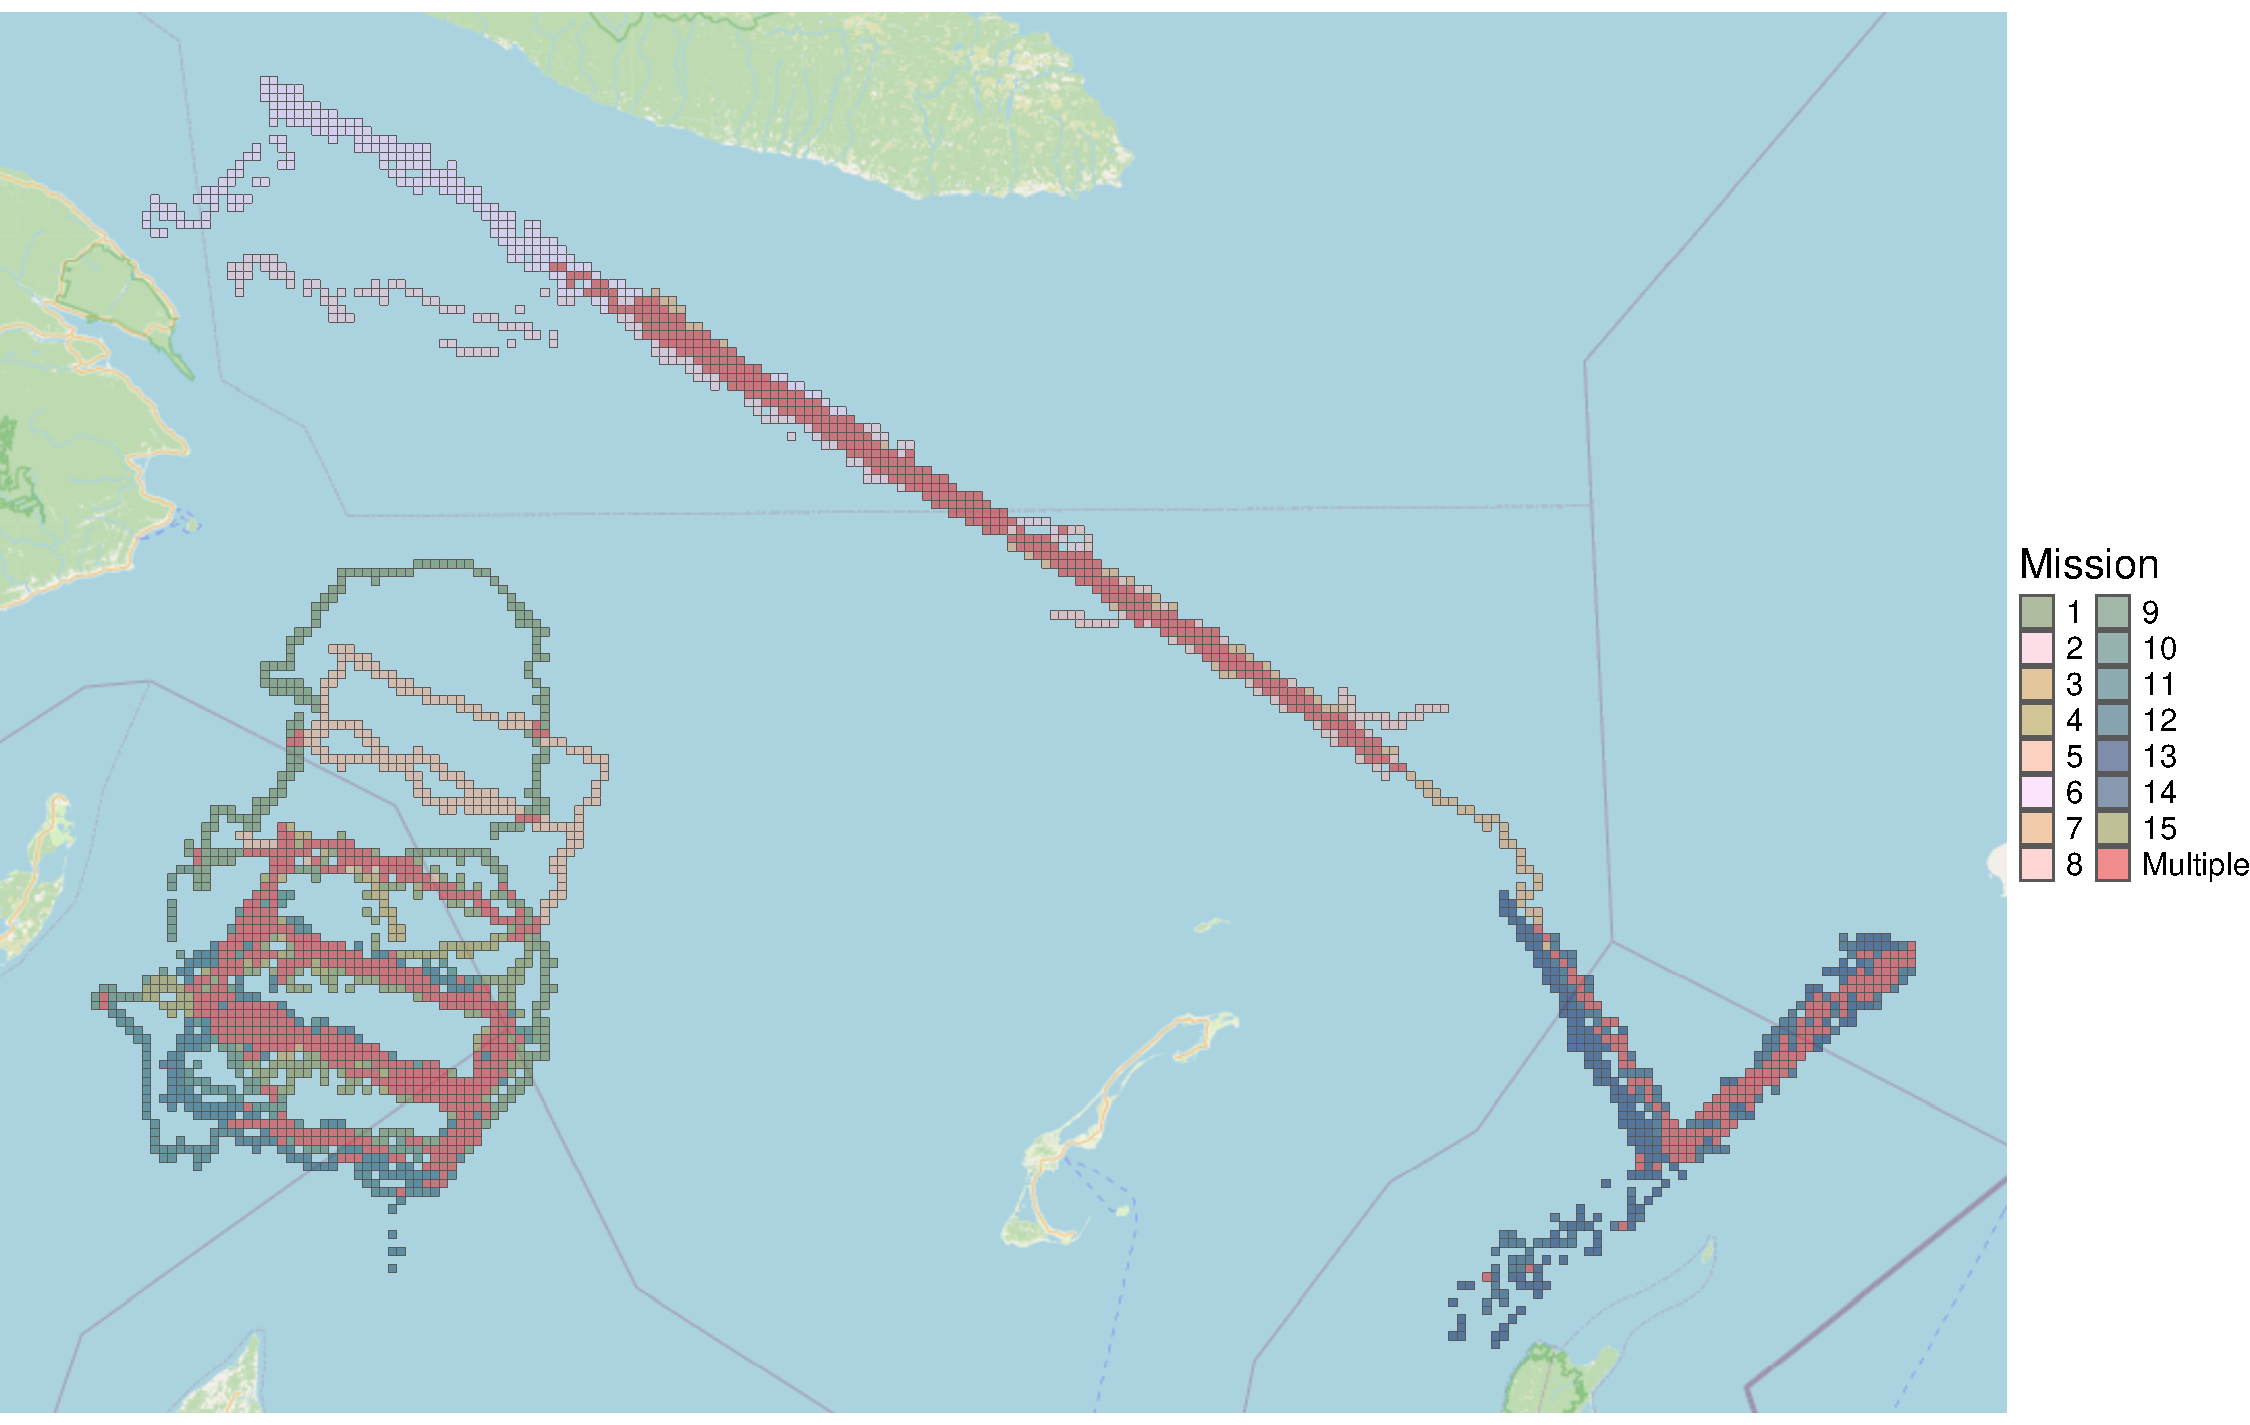
\includegraphics[width=0.9\textwidth]{Figures/Mission Map.pdf}  %\end{center}
  
\end{block}

\vspace{-15pt}

\begin{block}{Analysis}

\begin{columns}[t]
    \begin{column}{0.5 \colwidth}
    \vspace{-30pt}
    \heading{Regress Oxygen on Depth}
        \begin{itemize}
    \vspace{-15pt}
            \item Simple linear regression (simple)
            \item Smoothing spline (complex)
            \item Effect for mission
        \end{itemize}
    \end{column}

      \begin{column}{0.5 \colwidth}
    \vspace{-30pt}
      \heading{Compare Models}
      \begin{itemize}
    \vspace{-15pt}
          \item Degrees of Freedom (wiggliness) 
          \item Adjusted $R^2$ (quality of fit) 
          \item ANOVA
      \end{itemize}
      \end{column}
      
  \end{columns}

\vspace{10pt}
  
  \begin{columns}[t]
    \begin{column}{0.45 \colwidth}
    \begin{figure}
        \centering
      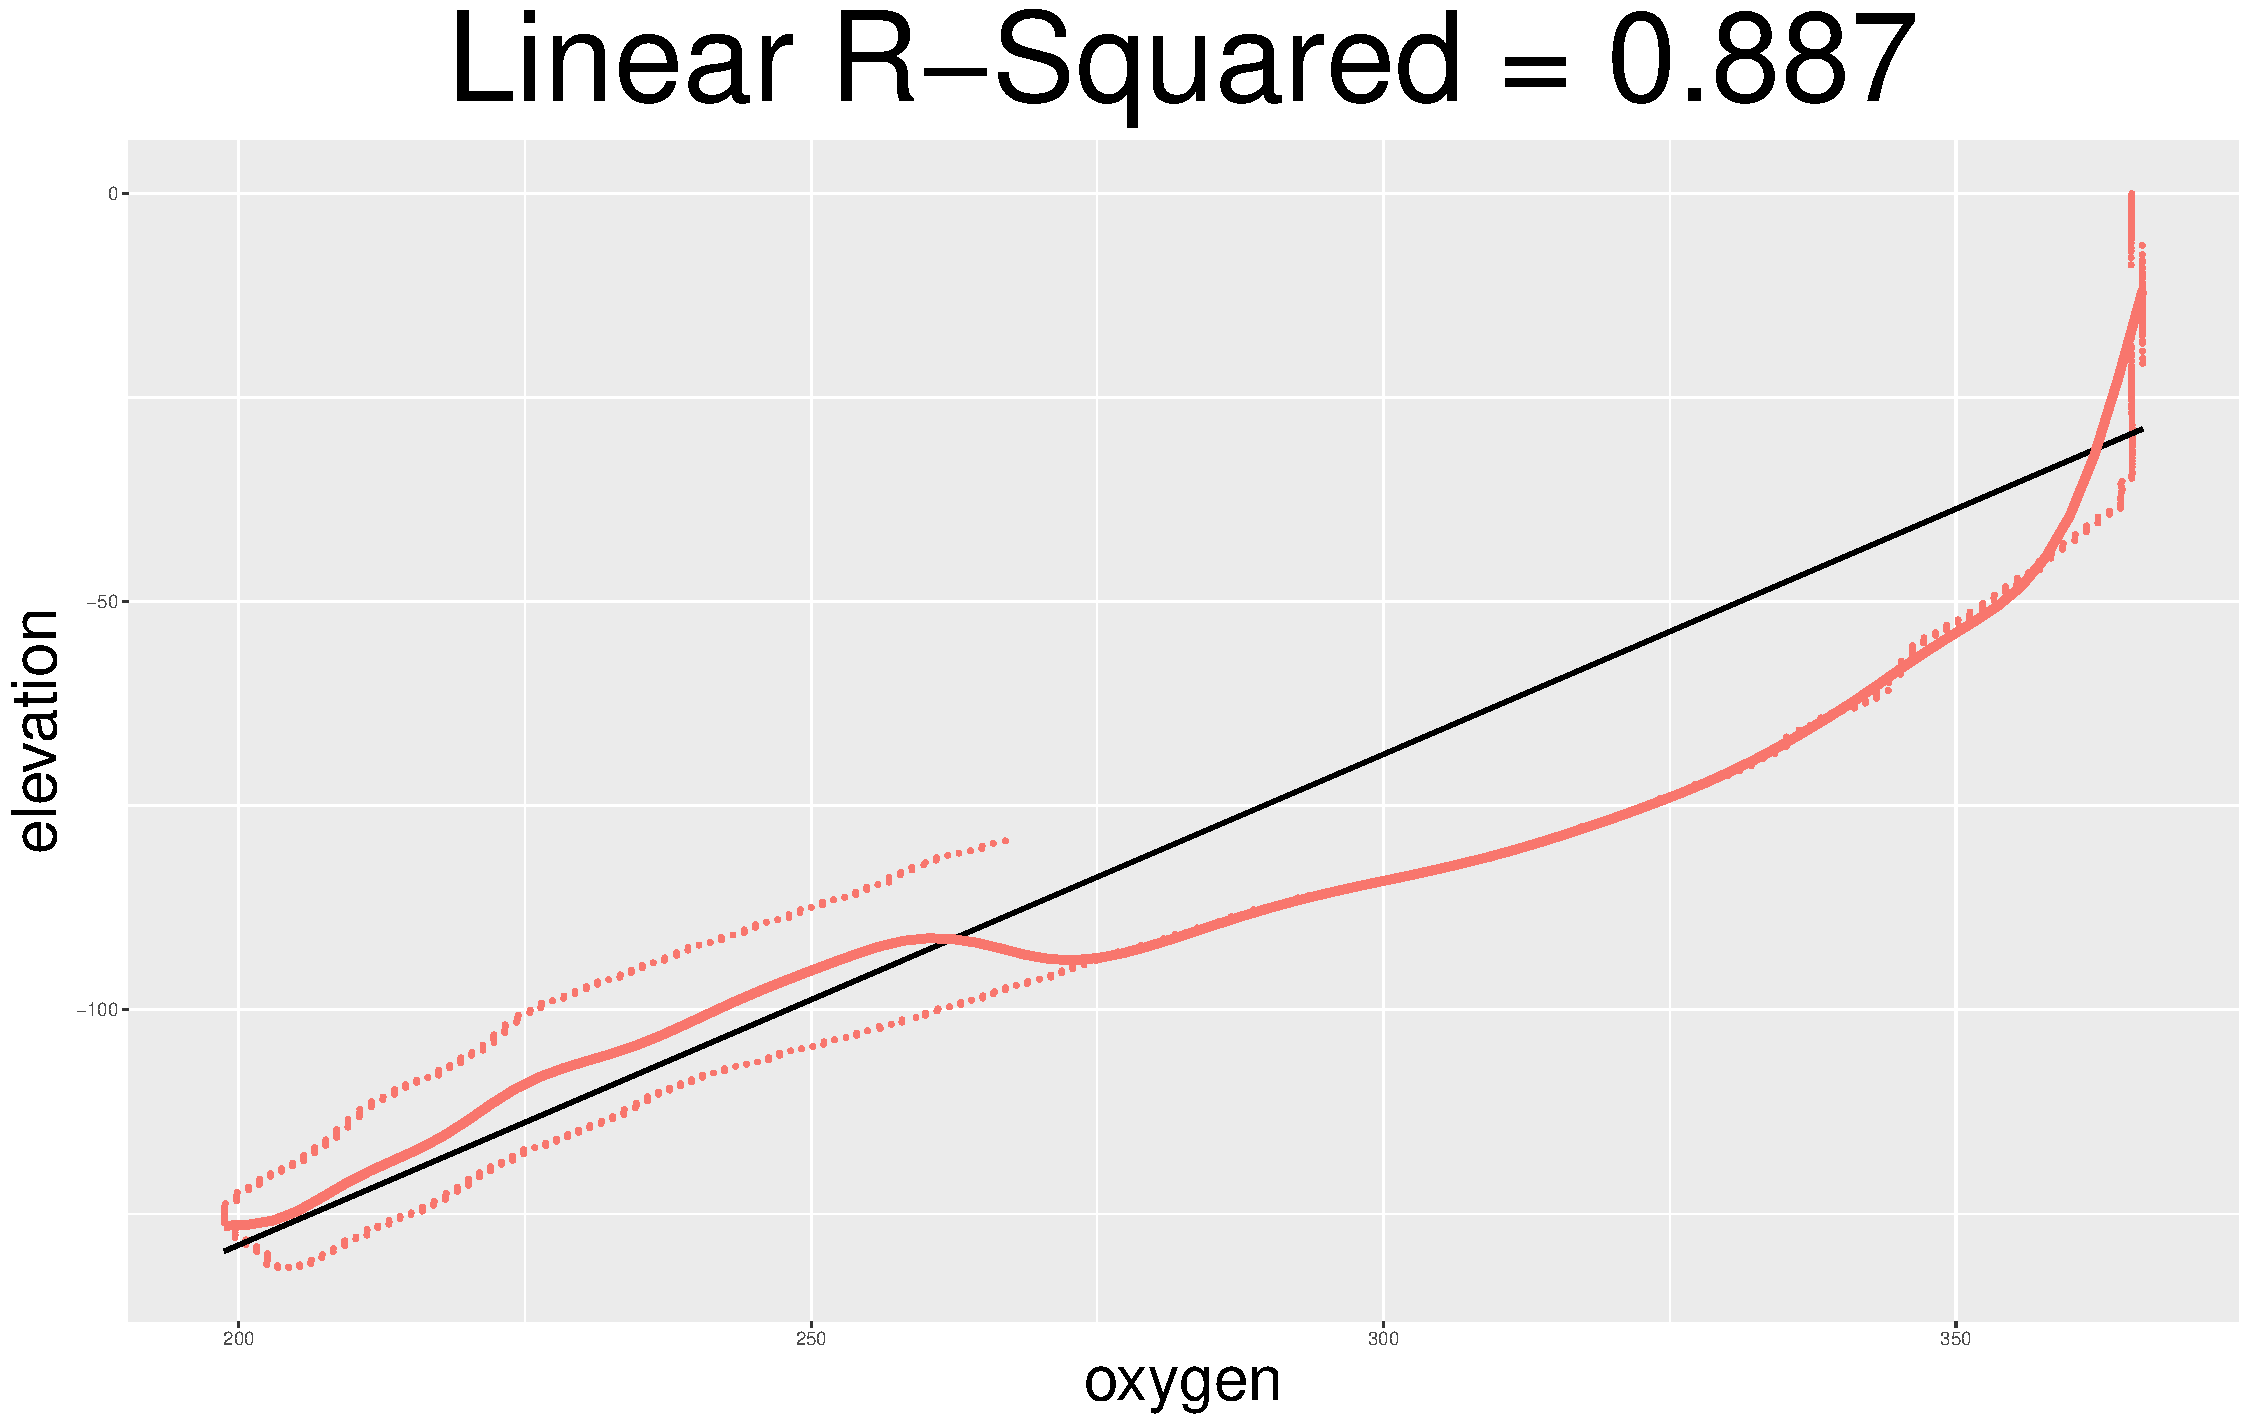
\includegraphics[width= \textwidth]{Figures/high_linear_R2.pdf}    
      \vspace{-60pt}
        \caption{Typical Low Complexity Region}
    \end{figure}
    \end{column}


      \begin{column}{0.45 \colwidth}
      \begin{figure}
        \centering
      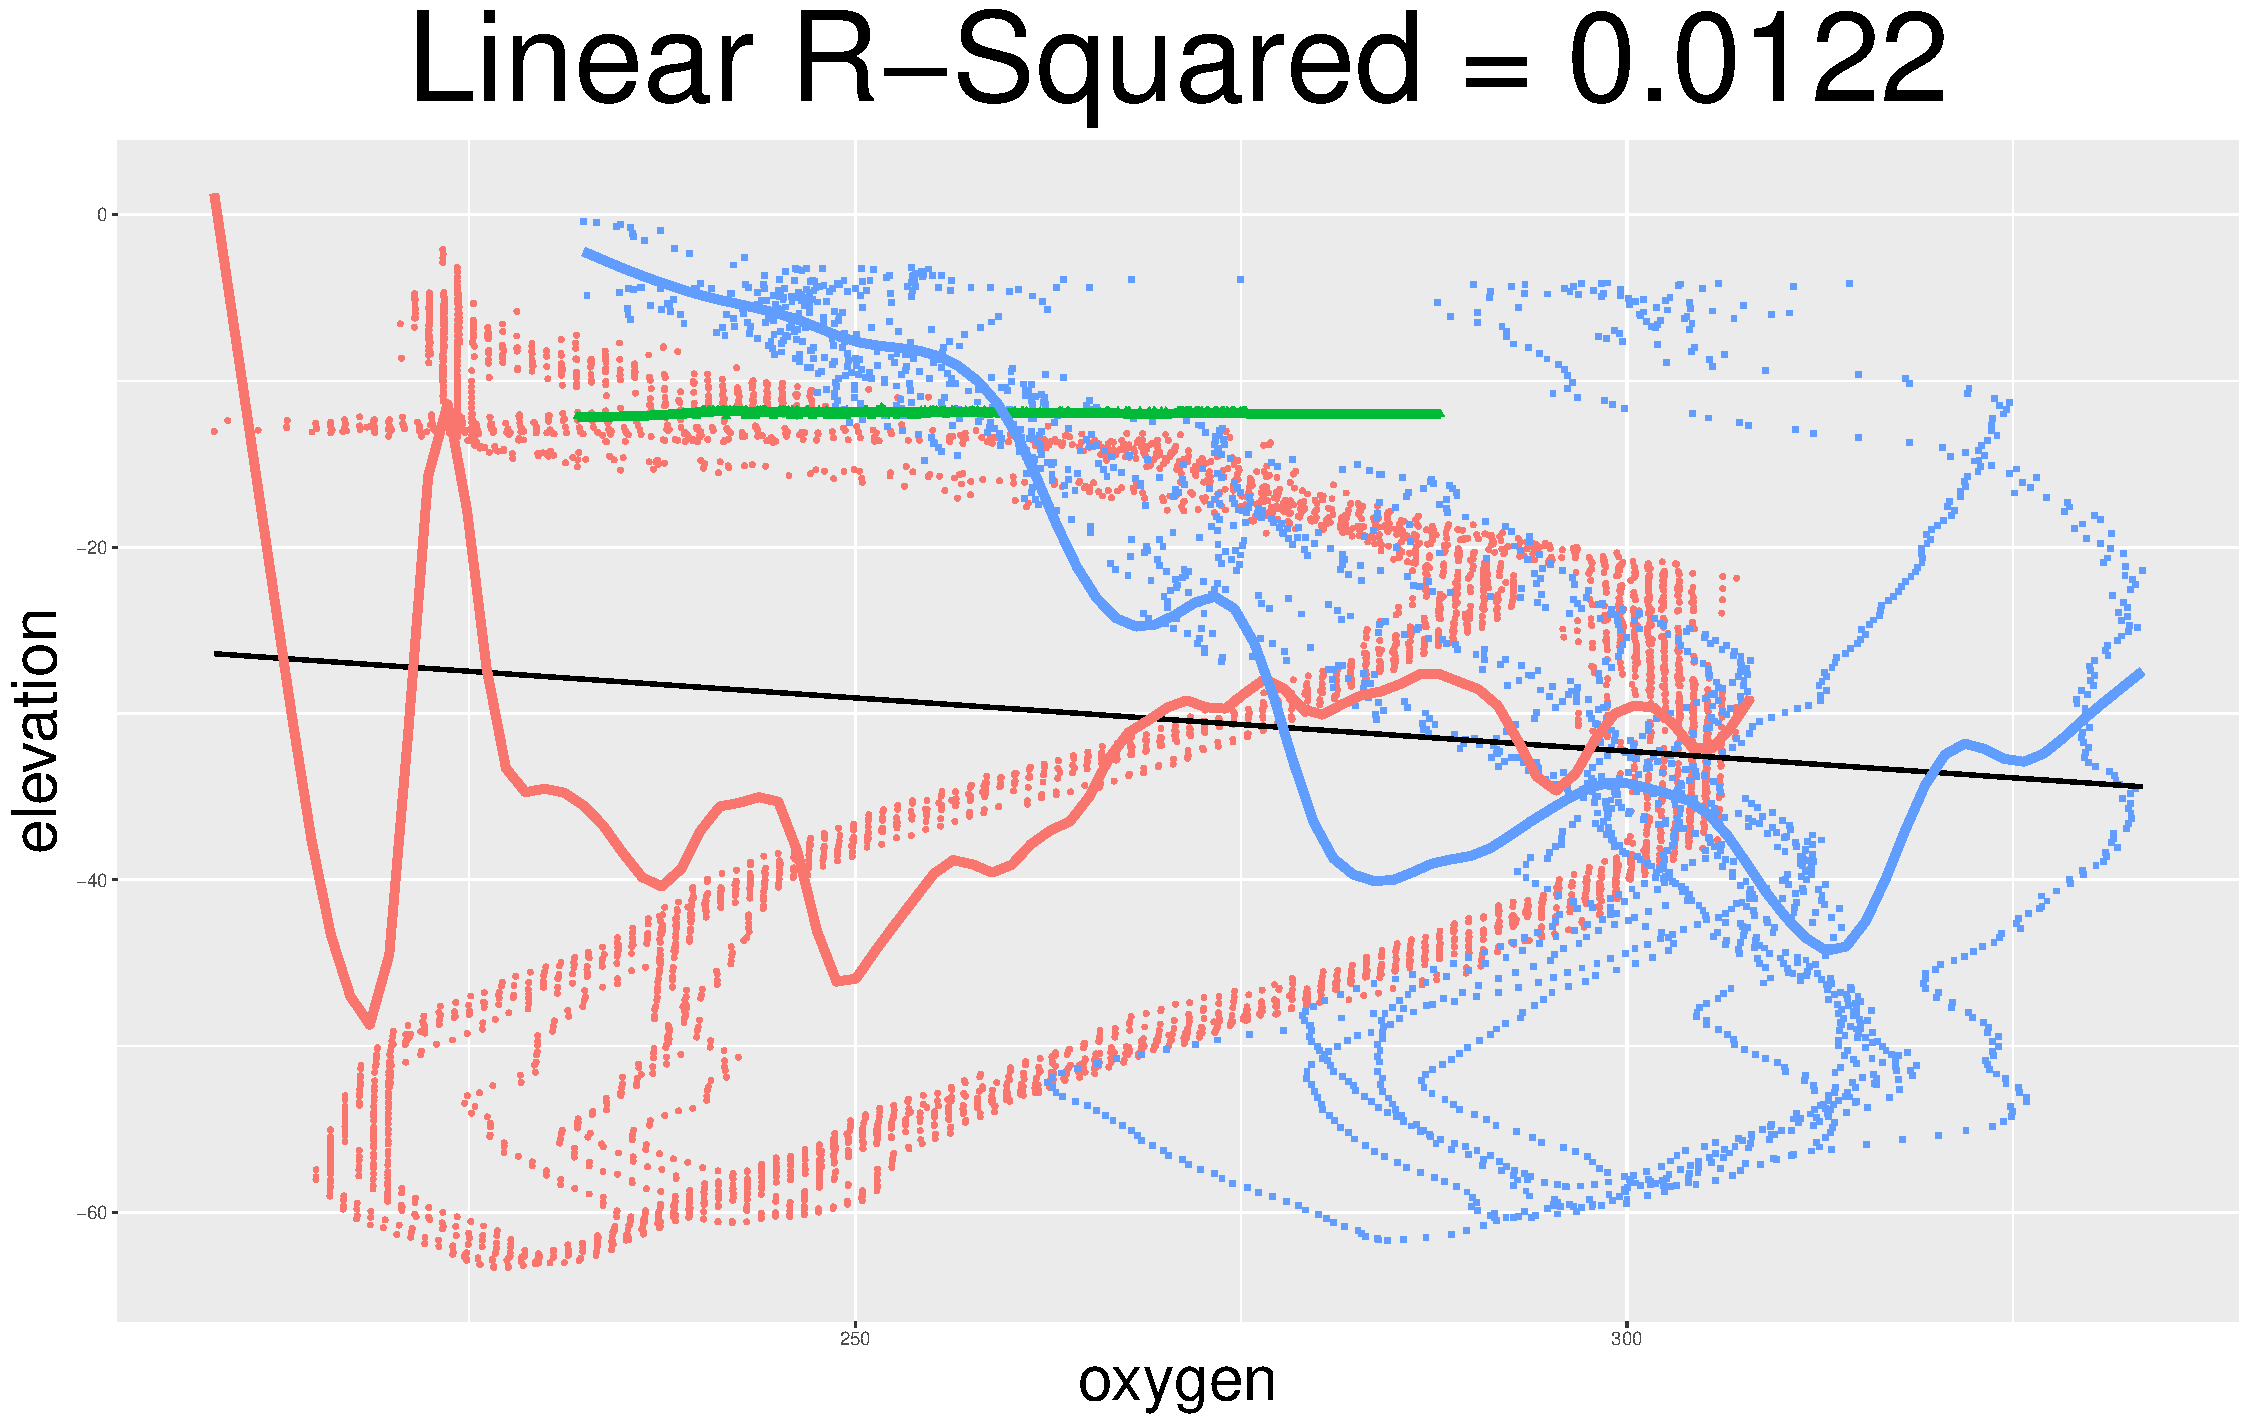
\includegraphics[width= \textwidth]{Figures/low_linear_R2.pdf}   
      \vspace{-60pt}
        \caption{Typical High Complexity Region}
    \end{figure}
      \end{column}
      
  \end{columns}
    

\end{block}

\end{column}

\separatorcolumn






\begin{column}{1.2\colwidth}
\vspace{-30pt}


  \begin{block}{Results}

  \begin{columns}[t]
      \begin{column}{0.48 \textwidth}
    \vspace{-30pt}
    \heading{Plots}
    \vspace{-10pt}
          \begin{itemize}
              \item Heterogeneous wiggliness
              \item Band of high DF in NW \newline
              \vspace{-20pt}
              \item Splines effective predictors
              \item Mission important for SW blob
              \item Some exceptional pockets
          \end{itemize}

        %  \vspace{-20pt}
      %\heading{ANOVA}
          
      \end{column}

      \begin{column}{0.48 \textwidth}
    \vspace{-20pt}
    \begin{flushright}
        
        \begin{figure}
          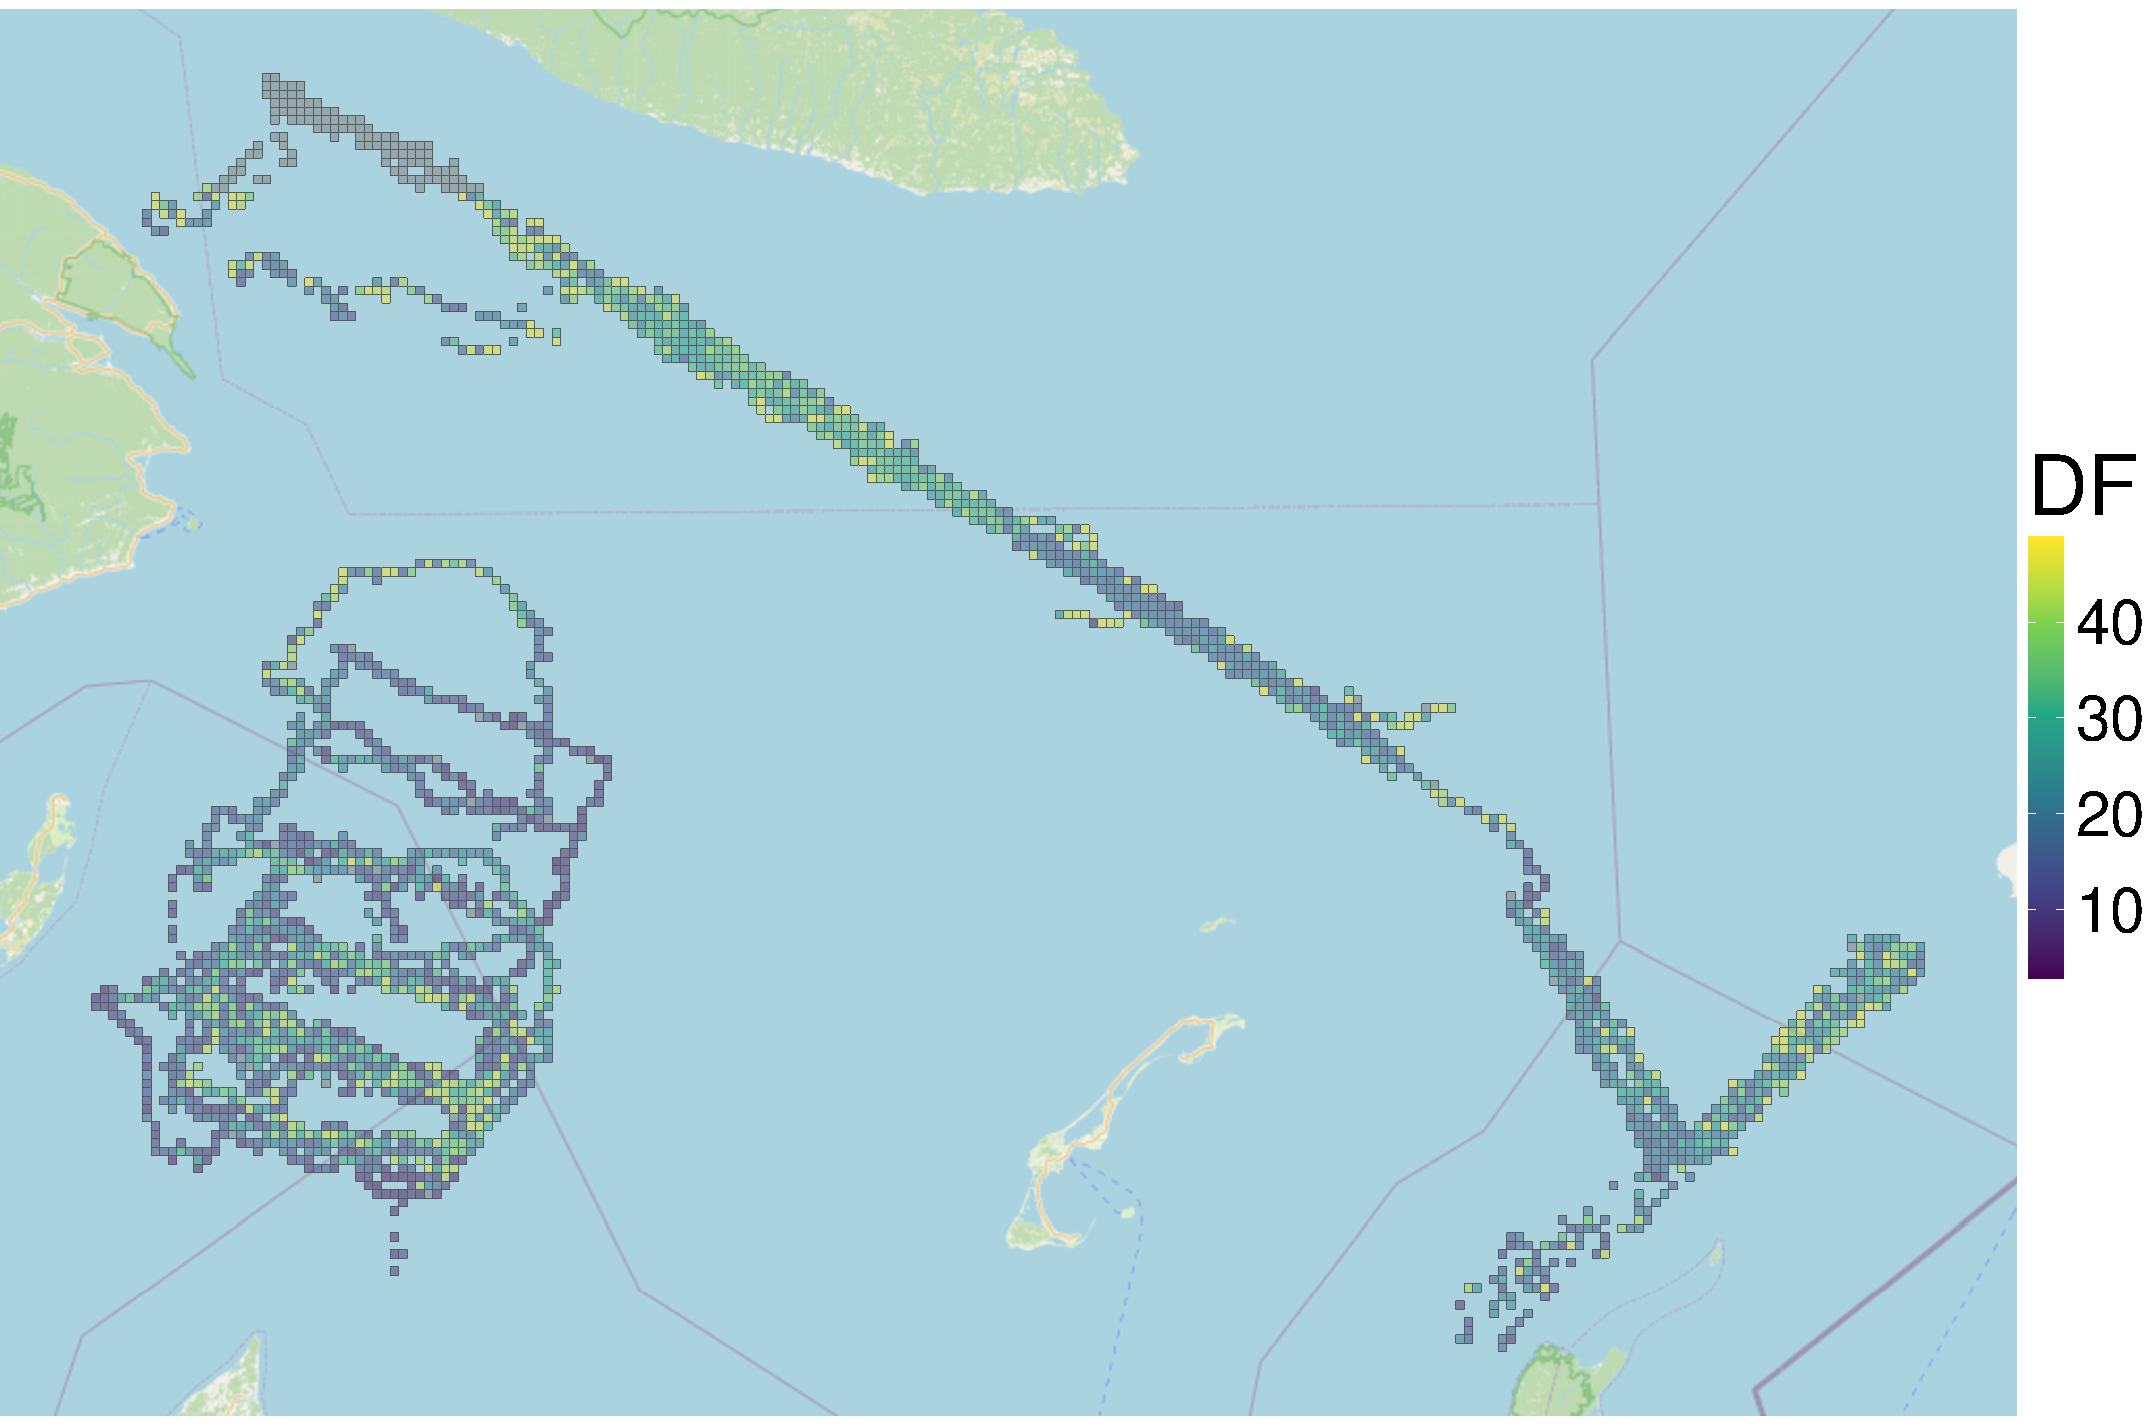
\includegraphics[width= \textwidth]{Figures/EDF Map.pdf}  
      \vspace{-55pt}
          \caption{Degrees of Freedom by Region}
        \end{figure}      
    \end{flushright}
        \end{column}
  \end{columns}

    \vspace{-50pt}
      \heading{ANOVA}
      \vspace{-20pt}
        \begin{itemize}
            \item No significant interaction between model and type of mission effect
            \item Mission significantly improves $R^2$, interaction effect marginal ($p \approx 0.02$)
            \item No significant differences between mission effect types for DF
        \end{itemize}

    \vspace{-10pt}
    
\begin{figure}
\begin{center}
    \centering
    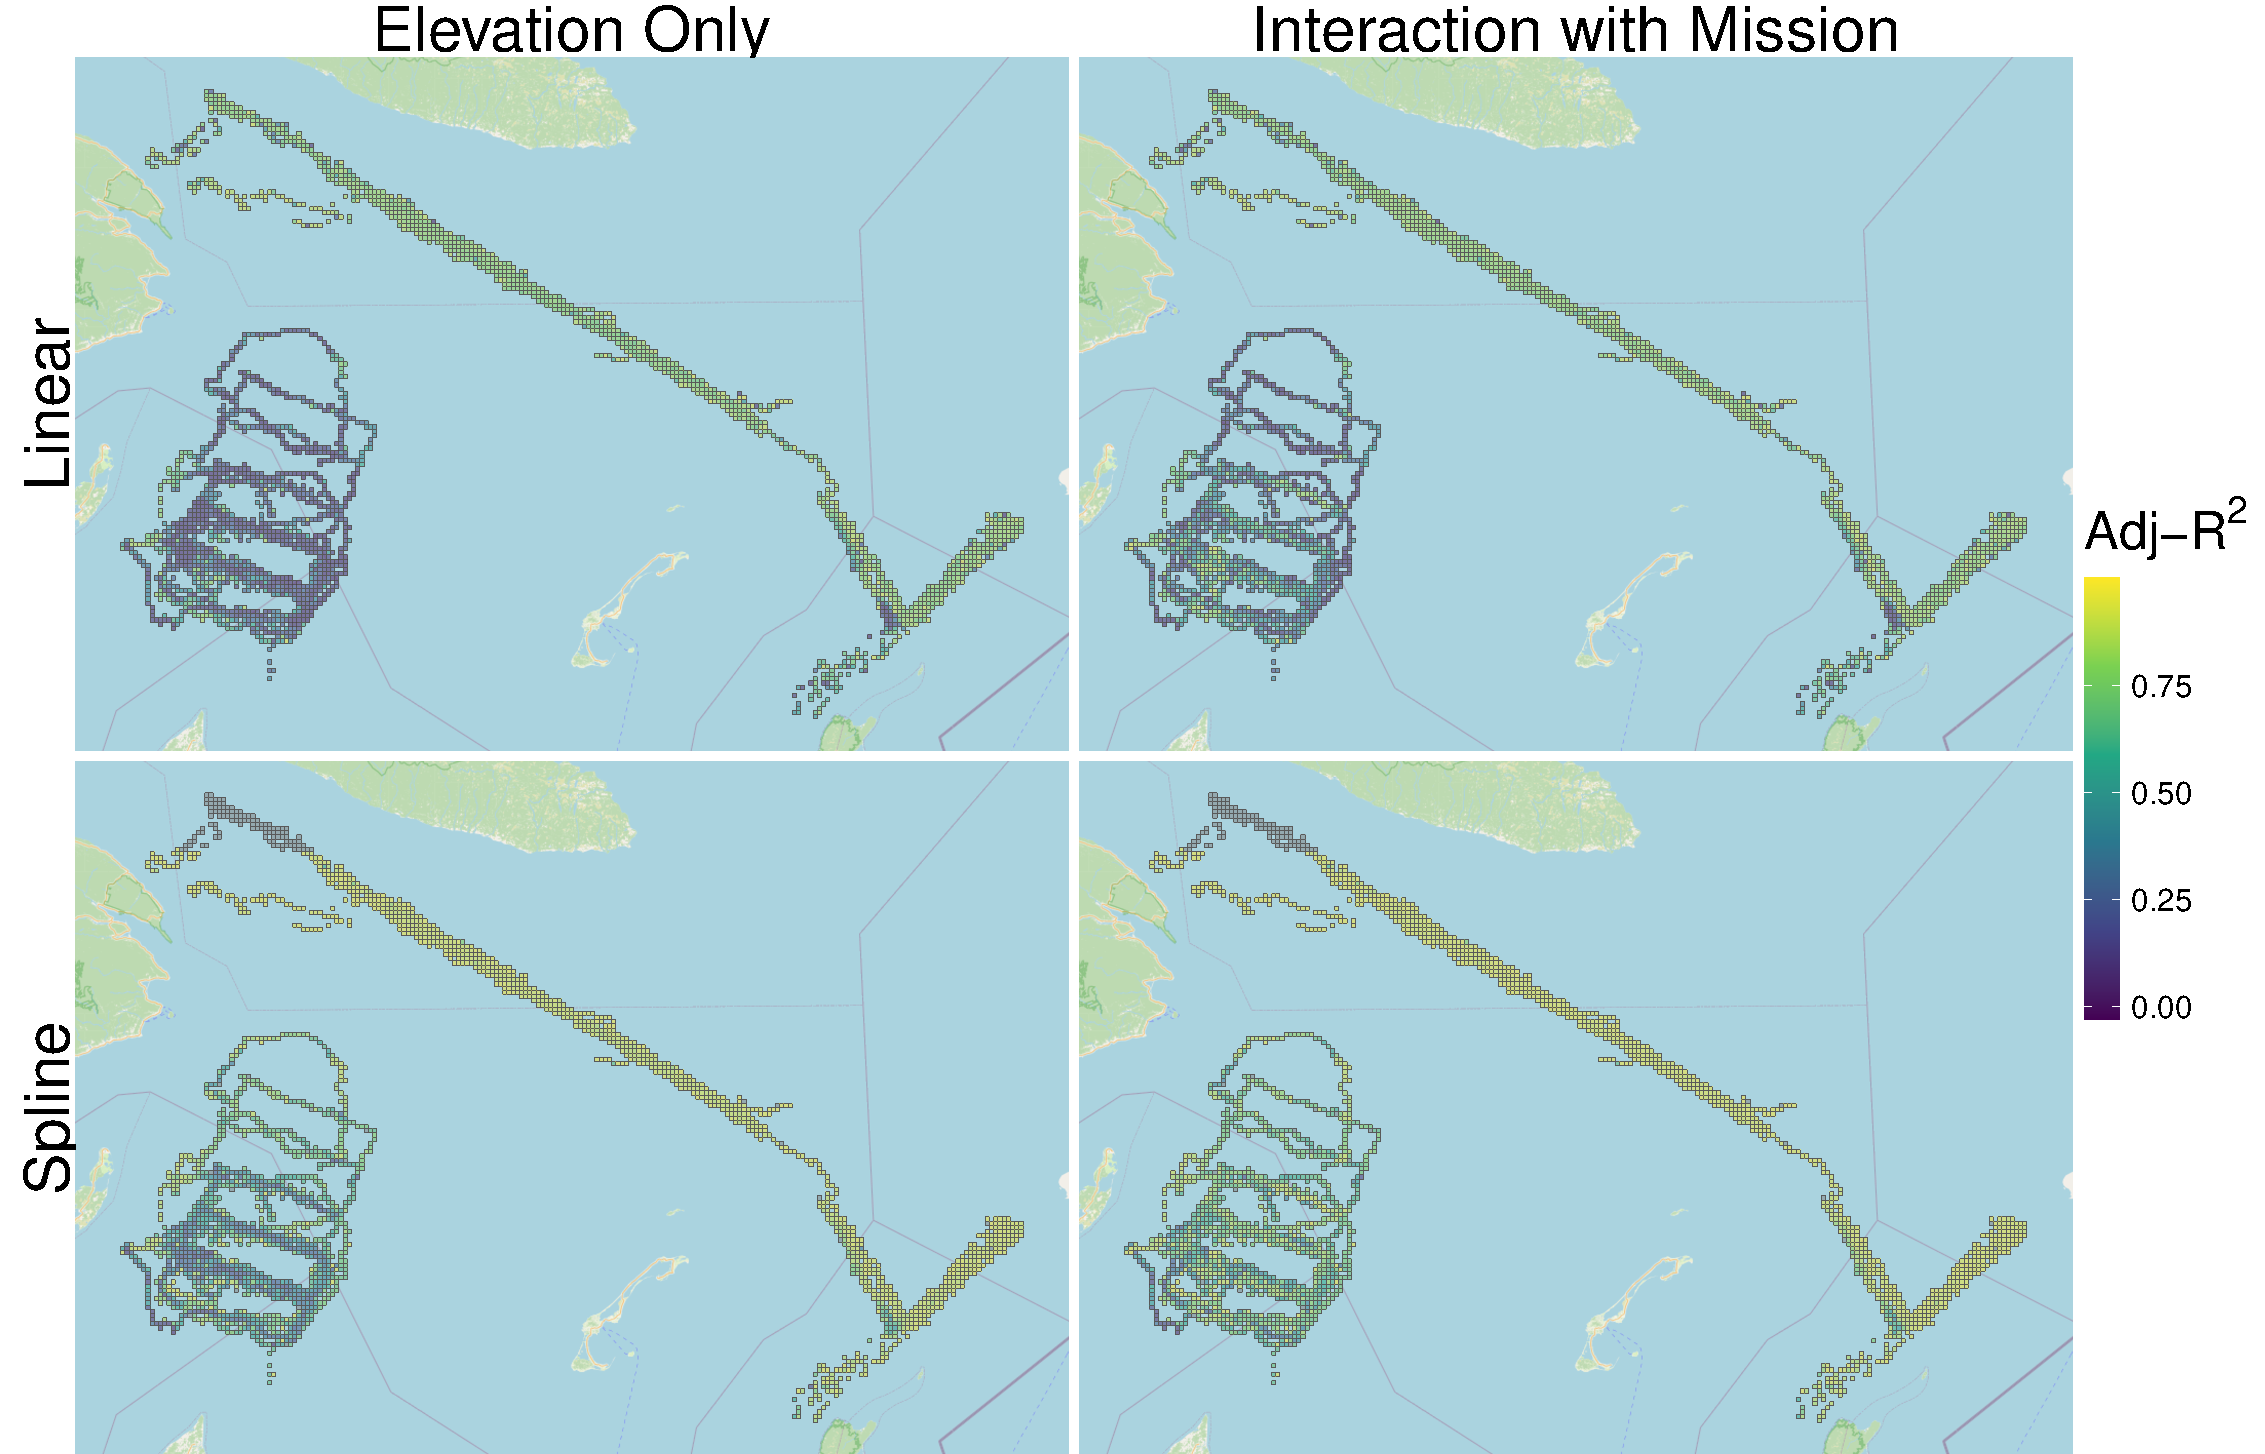
\includegraphics[width=0.92\textwidth]{Figures/R2 Map.pdf}
    \vspace{-25pt}
    \caption{Adjusted R-Squared by Region}
\end{center}
\end{figure}

  \end{block}


\end{column}

\separatorcolumn





\begin{column}{0.8\colwidth}
\vspace{-30pt}

\begin{block}{Discussion}
    \vspace{-15pt}

    \heading{Our Contribution}
    \vspace{-25pt}
    \begin{itemize}
        \item We identified some complicated regions for further investigation
        \item Our approach can easily be modified to use a different baseline (simple) model
        \begin{itemize}
            \item E.g. One that incorporates existing knowledge about ocean dynamics
        \end{itemize}
    \end{itemize}

\vspace{-25pt}

    \heading{Future Work}
    \vspace{-25pt}
    \begin{itemize}
        \item More principled approach for temporal dynamics
        \item Incorporate other covariates and ship data
        \item Model underwater position of glider
    \end{itemize}
\end{block}

\vspace{-30pt}

\begin{block}{Acknowledgments}
      We would like to thank Jaclyn Ruth and Gareth Wolff for their helpful input, our faculty mentor, Bouchra Nasri, and the following agencies for their financial support:  
    
    
\includegraphics[width=0.2\colwidth]{logos/CANSSI_Logo.png}
    
\includegraphics[width=0.3\colwidth]{logos/CIHR_logo.jpg}
    
\includegraphics[width=0.25\colwidth]{logos/NSERC_Logo.png}

      
\end{block}

\vspace{-15pt}

\begin{block}{More Information}

\begin{columns}[t]
    \begin{column}{0.45 \colwidth}
    \vspace{-20pt}
    \begin{figure}
        \centering
    \qrcode[height=4cm]{https://github.com/wruth1/SSC-2025-Case-Study}
    \vspace{-10pt}
        \caption{GitHub Repository}
    \end{figure}
    \end{column}


      \begin{column}{0.45 \colwidth}
    \vspace{-20pt}
      \begin{figure}
        \centering
    \qrcode[height=4cm]{mailto:william.ruth@umontreal.ca}
      \vspace{-10pt}
        \caption{Email Us}
    \end{figure}
      \end{column}
      
  \end{columns}


    
\end{block}

  

\end{column}

\separatorcolumn
\end{columns}
\end{frame}

\end{document}
